%%%%%%%%%%%%%%%%%%%%%%%%%%%%%%%%%%%%%%%%%
% The Legrand Orange Book
% LaTeX Template
% Version 1.4 (12/4/14)
%
% This template has been downloaded from:
% http://www.LaTeXTemplates.com
%
% Original author:
% Mathias Legrand (legrand.mathias@gmail.com)
%
% License:
% CC BY-NC-SA 3.0 (http://creativecommons.org/licenses/by-nc-sa/3.0/)
%
% Compiling this template:
% This template uses biber for its bibliography and makeindex for its index.
% When you first open the template, compile it from the command line with the 
% commands below to make sure your LaTeX distribution is configured correctly:
%
% 1) pdflatex main
% 2) makeindex main.idx -s StyleInd.ist
% 3) biber main
% 4) pdflatex main x 2
%
% After this, when you wish to update the bibliography/index use the appropriate
% command above and make sure to compile with pdflatex several times 
% afterwards to propagate your changes to the document.
%
% This template also uses a number of packages which may need to be
% updated to the newest versions for the template to compile. It is strongly
% recommended you update your LaTeX distribution if you have any
% compilation errors.
%
% Important note:
% Chapter heading images should have a 2:1 width:height ratio,
% e.g. 920px width and 460px height.
%
%%%%%%%%%%%%%%%%%%%%%%%%%%%%%%%%%%%%%%%%%

%----------------------------------------------------------------------------------------
%	PACKAGES AND OTHER DOCUMENT CONFIGURATIONS
%----------------------------------------------------------------------------------------

\documentclass[11pt,fleqn]{book} % Default font size and left-justified equations

\usepackage[top=3cm,bottom=3cm,left=3.2cm,right=3.2cm,headsep=10pt,a4paper]{geometry} % Page margins

\usepackage{xcolor} % Required for specifying colors by name
\definecolor{ocre}{RGB}{243,102,25} % Define the orange color used for highlighting throughout the book

% Font Settings
\usepackage{avant} % Use the Avantgarde font for headings
%\usepackage{times} % Use the Times font for headings
\usepackage{mathptmx} % Use the Adobe Times Roman as the default text font together with math symbols from the Sym­bol, Chancery and Com­puter Modern fonts

\usepackage{microtype} % Slightly tweak font spacing for aesthetics
\usepackage[utf8]{inputenc} % Required for including letters with accents
\usepackage[T1]{fontenc} % Use 8-bit encoding that has 256 glyphs

% Bibliography
%\usepackage[style=alphabetic,sorting=nyt,sortcites=true,autopunct=true,babel=hyphen,hyperref=true,abbreviate=false,backref=true,backend=biber]{biblatex}
\usepackage[style=alphabetic,sorting=nyt,sortcites=true,autopunct=true,babel=hyphen,hyperref=true,abbreviate=false,backref=true,backend=bibtex]{biblatex}
\addbibresource{bibliography.bib} % BibTeX bibliography file
\defbibheading{bibempty}{}

% Index
\usepackage{calc} % For simpler calculation - used for spacing the index letter headings correctly
\usepackage{makeidx} % Required to make an index
\makeindex % Tells LaTeX to create the files required for indexing

%Codes
\usepackage{listings}
\usepackage{color}

\definecolor{mygreen}{rgb}{0,0.6,0}
\definecolor{mygray}{rgb}{0.5,0.5,0.5}
\definecolor{mymauve}{rgb}{0.58,0,0.82}

%----------------------------------------------------------------------------------------

%#COLORS
\definecolor{color1}{RGB}{163,99,226} %#9363DE Texto violeta
\definecolor{color2}{RGB}{233,147,109} % PRODUCTO DE CALIDAD
\definecolor{color3}{RGB}{255,243,235} % PRODUCTO DE CALIDAD
\definecolor{colorTEXT}{RGB}{47,47,47} % TEX
\definecolor{colorT1}{RGB}{134,161,220} % TEORIA
\definecolor{colorT2}{RGB}{234,239,255} % TEORIA
\definecolor{colorE1}{RGB}{0,205,132} % EJEMPLO
\definecolor{colorE2}{RGB}{227,255,238} % EJEMPLO
\definecolor{colorA1}{RGB}{233,147,109} % ALERTA
\definecolor{colorA2}{RGB}{255,243,235} % ALERTA
\definecolor{colorIN1}{RGB}{255,195,138} % INPUTS
\definecolor{colorIN2}{RGB}{255,237,219} % INPUTS
\definecolor{colorAS1}{RGB}{255,172,163} % ESTADO PRESENTE/ACTUAL
\definecolor{colorAS2}{RGB}{255,229,227} % ESTADO PRESENTE/ACTUAL
\definecolor{colorFS1}{RGB}{203,158,198} % ESTADO FUTURO
\definecolor{colorFS2}{RGB}{240,225,237} % ESTADO FUTURO
\definecolor{colorFF1}{RGB}{92,201,226} % FLIP-FLOPS
\definecolor{colorFF2}{RGB}{209,238,246} % FLIP-FLOPS
\definecolor{colorOUT1}{RGB}{142,150,218} % SALIDAS
\definecolor{colorOUT2}{RGB}{220,223,243} % SALIDAS

%----------------------------------------------------------------------------------------
%	VARIOUS REQUIRED PACKAGES
%----------------------------------------------------------------------------------------

\usepackage{titlesec} % Allows customization of titles

\usepackage{graphicx} % Required for including pictures
\graphicspath{{Pictures/}} % Specifies the directory where pictures are stored

\usepackage{lipsum} % Inserts dummy text

\usepackage{tikz} % Required for drawing custom shapes

\usepackage[english]{babel} % English language/hyphenation

\usepackage{enumitem} % Customize lists
\setlist{nolistsep} % Reduce spacing between bullet points and numbered lists

\usepackage{booktabs} % Required for nicer horizontal rules in tables

\usepackage{eso-pic} % Required for specifying an image background in the title page

%----------------------------------------------------------------------------------------
%	MAIN TABLE OF CONTENTS
%----------------------------------------------------------------------------------------

\usepackage{titletoc} % Required for manipulating the table of contents

\contentsmargin{0cm} % Removes the default margin
% Chapter text styling
\titlecontents{chapter}[1.25cm] % Indentation
{\addvspace{15pt}\large\sffamily\bfseries} % Spacing and font options for chapters
{\color{color2!60}\contentslabel[\Large\thecontentslabel]{1.25cm}\color{color2}} % Chapter number
{}  
{\color{color2!60}\normalsize\sffamily\bfseries\;\titlerule*[.5pc]{.}\;\thecontentspage} % Page number
% Section text styling
\titlecontents{section}[1.25cm] % Indentation
{\addvspace{5pt}\sffamily\bfseries} % Spacing and font options for sections
{\contentslabel[\thecontentslabel]{1.25cm}} % Section number
{}
{\sffamily\hfill\color{black}\thecontentspage} % Page number
[]
% Subsection text styling
\titlecontents{subsection}[1.25cm] % Indentation
{\addvspace{1pt}\sffamily\small} % Spacing and font options for subsections
{\contentslabel[\thecontentslabel]{1.25cm}} % Subsection number
{}
{\sffamily\;\titlerule*[.5pc]{.}\;\thecontentspage} % Page number
[] 

%----------------------------------------------------------------------------------------
%	MINI TABLE OF CONTENTS IN CHAPTER HEADS
%----------------------------------------------------------------------------------------

% Section text styling
\titlecontents{lsection}[0em] % Indendating
{\footnotesize\sffamily} % Font settings
{}
{}
{}

% Subsection text styling
\titlecontents{lsubsection}[.5em] % Indentation
{\normalfont\footnotesize\sffamily} % Font settings
{}
{}
{}
 
%----------------------------------------------------------------------------------------
%	PAGE HEADERS
%----------------------------------------------------------------------------------------
\addto\captionsenglish{%
  \renewcommand\chaptername{\textbf{Capítulo}}}
  
\usepackage{fancyhdr} % Required for header and footer configuration

\pagestyle{fancy}
\renewcommand{\chaptermark}[1]{\markboth{\sffamily\scriptsize\chaptername\ \textbf{\thechapter.}\ #1}{}} % Chapter text font settings
\renewcommand{\sectionmark}[1]{\markright{\sffamily\scriptsize\thesection\hspace{5pt}#1}{}} % Section text font settings
\fancyhf{} \fancyhead[LE,RO]{\sffamily\scriptsize\thepage} % Font setting for the page number in the header
\fancyhead[LO]{\nouppercase \rightmark} % Print the nearest section name on the left side of odd pages
\fancyhead[RE]{\nouppercase \leftmark} % Print the current chapter name on the right side of even pages
\renewcommand{\headrulewidth}{0.5pt} % Width of the rule under the header
\addtolength{\headheight}{2.5pt} % Increase the spacing around the header slightly
\renewcommand{\footrulewidth}{1pt} % Removes the rule in the footer
\fancypagestyle{plain}{\fancyhead{}\renewcommand{\headrulewidth}{0pt}} % Style for when a plain pagestyle is specified
\fancyfoot[CE,CO]{\begin{picture}(0,0) \put(0,-5){\includegraphics[width=2.5cm]{./Pictures/LogoCC1.png}} \end{picture} \hspace{10cm} \scriptsize{F.Segura-Quijano y C.Quintero Peña}}
\lhead{\begin{picture}(0,0) \put(0,0){\includegraphics[width=0.7cm]{./Pictures/LogoUniandes.pdf}} \end{picture} } % \hspace{0.7cm} Universidad de los Andes - Colombia}

%\begin{picture}(0,0) \put(0,0){\includegraphics[width=0.7cm]{./Pictures/LogoUniandes.pdf}} \end{picture}

% Removes the header from odd empty pages at the end of chapters
\makeatletter
\renewcommand{\cleardoublepage}{
\clearpage\ifodd\c@page\else
\hbox{}
\vspace*{\fill}
\thispagestyle{empty}
\newpage
\fi}

%----------------------------------------------------------------------------------------
%	THEOREM STYLES
%----------------------------------------------------------------------------------------

\usepackage{amsmath,amsfonts,amssymb,amsthm} % For math equations, theorems, symbols, etc

\newcommand{\intoo}[2]{\mathopen{]}#1\,;#2\mathclose{[}}
\newcommand{\ud}{\mathop{\mathrm{{}d}}\mathopen{}}
\newcommand{\intff}[2]{\mathopen{[}#1\,;#2\mathclose{]}}
\newtheorem{notation}{Notation}[chapter]

%%%%%%%%%%%%%%%%%%%%%%%%%%%%%%%%%%%%%%%%%%%%%%%%%%%%%%%%%%%%%%%%%%%%%%%%%%%
%%%%%%%%%%%%%%%%%%%% dedicated to boxed/framed environements %%%%%%%%%%%%%%
%%%%%%%%%%%%%%%%%%%%%%%%%%%%%%%%%%%%%%%%%%%%%%%%%%%%%%%%%%%%%%%%%%%%%%%%%%%
\newtheoremstyle{ocrenumbox}% % Theorem style name
{0pt}% Space above
{0pt}% Space below
{\normalfont}% % Body font
{}% Indent amount
{\small\bf\sffamily\color{ocre}}% % Theorem head font
{\;}% Punctuation after theorem head
{0.25em}% Space after theorem head
{\small\sffamily\color{ocre}\thmname{#1}\nobreakspace\thmnumber{\@ifnotempty{#1}{}\@upn{#2}}% Theorem text (e.g. Theorem 2.1)
\thmnote{\nobreakspace\the\thm@notefont\sffamily\bfseries\color{black}---\nobreakspace#3.}} % Optional theorem note
\renewcommand{\qedsymbol}{$\blacksquare$}% Optional qed square

\newtheoremstyle{blacknumex}% Theorem style name
{5pt}% Space above
{5pt}% Space below
{\normalfont}% Body font
{} % Indent amount
{\small\bf\sffamily}% Theorem head font
{\;}% Punctuation after theorem head
{0.25em}% Space after theorem head
{\small\sffamily{\tiny\ensuremath{\blacksquare}}\nobreakspace\thmname{#1}\nobreakspace\thmnumber{\@ifnotempty{#1}{}\@upn{#2}}% Theorem text (e.g. Theorem 2.1)
\thmnote{\nobreakspace\the\thm@notefont\sffamily\bfseries---\nobreakspace#3.}}% Optional theorem note

\newtheoremstyle{blacknumbox} % Theorem style name
{0pt}% Space above
{0pt}% Space below
{\normalfont}% Body font
{}% Indent amount
{\small\bf\sffamily}% Theorem head font
{\;}% Punctuation after theorem head
{0.25em}% Space after theorem head
{\small\sffamily\thmname{#1}\nobreakspace\thmnumber{\@ifnotempty{#1}{}\@upn{#2}}% Theorem text (e.g. Theorem 2.1)
\thmnote{\nobreakspace\the\thm@notefont\sffamily\bfseries---\nobreakspace#3.}}% Optional theorem note

%%%%%%%%%%%%%%%%%%%%%%%%%%%%%%%%%%%%%%%%%%%%%%%%%%%%%%%%%%%%%%%%%%%%%%%%%%%
%%%%%%%%%%%%% dedicated to non-boxed/non-framed environements %%%%%%%%%%%%%
%%%%%%%%%%%%%%%%%%%%%%%%%%%%%%%%%%%%%%%%%%%%%%%%%%%%%%%%%%%%%%%%%%%%%%%%%%%
\newtheoremstyle{ocrenum}% % Theorem style name
{5pt}% Space above
{5pt}% Space below
{\normalfont}% % Body font
{}% Indent amount
{\small\bf\sffamily\color{ocre}}% % Theorem head font
{\;}% Punctuation after theorem head
{0.25em}% Space after theorem head
{\small\sffamily\color{ocre}\thmname{#1}\nobreakspace\thmnumber{\@ifnotempty{#1}{}\@upn{#2}}% Theorem text (e.g. Theorem 2.1)
\thmnote{\nobreakspace\the\thm@notefont\sffamily\bfseries\color{black}---\nobreakspace#3.}} % Optional theorem note
\renewcommand{\qedsymbol}{$\blacksquare$}% Optional qed square
\makeatother

% Defines the theorem text style for each type of theorem to one of the three styles above
\newcounter{dummy} 
\numberwithin{dummy}{section}
\theoremstyle{ocrenumbox}
\newtheorem{theoremeT}[dummy]{Theorem}
\newtheorem{problem}{Problem}[chapter]
\newtheorem{exerciseT}{Exercise}[chapter]
\theoremstyle{blacknumex}
\newtheorem{exampleT}{Example}[chapter]
\theoremstyle{blacknumbox}
\newtheorem{vocabulary}{Vocabulary}[chapter]
\newtheorem{definitionT}{Definition}[section]
\newtheorem{corollaryT}[dummy]{Corollary}
\theoremstyle{ocrenum}
\newtheorem{proposition}[dummy]{Proposition}

%----------------------------------------------------------------------------------------
%	DEFINITION OF COLORED BOXES
%----------------------------------------------------------------------------------------

\RequirePackage[framemethod=default]{mdframed} % Required for creating the theorem, definition, exercise and corollary boxes

% Theorem box
\newmdenv[skipabove=7pt,
skipbelow=7pt,
backgroundcolor=black!5,
linecolor=ocre,
innerleftmargin=5pt,
innerrightmargin=5pt,
innertopmargin=5pt,
leftmargin=0cm,
rightmargin=0cm,
innerbottommargin=5pt]{tBox}

% Exercise box	  
\newmdenv[skipabove=7pt,
skipbelow=7pt,
rightline=false,
leftline=true,
topline=false,
bottomline=false,
backgroundcolor=ocre!10,
linecolor=ocre,
innerleftmargin=5pt,
innerrightmargin=5pt,
innertopmargin=5pt,
innerbottommargin=5pt,
leftmargin=0cm,
rightmargin=0cm,
linewidth=4pt]{eBox}	

% Definition box
\newmdenv[skipabove=7pt,
skipbelow=7pt,
rightline=false,
leftline=true,
topline=false,
bottomline=false,
linecolor=ocre,
innerleftmargin=5pt,
innerrightmargin=5pt,
innertopmargin=0pt,
leftmargin=0cm,
rightmargin=0cm,
linewidth=4pt,
innerbottommargin=0pt]{dBox}	

% Corollary box
\newmdenv[skipabove=7pt,
skipbelow=7pt,
rightline=false,
leftline=true,
topline=false,
bottomline=false,
linecolor=gray,
backgroundcolor=black!5,
innerleftmargin=5pt,
innerrightmargin=5pt,
innertopmargin=5pt,
leftmargin=0cm,
rightmargin=0cm,
linewidth=4pt,
innerbottommargin=5pt]{cBox}

% Creates an environment for each type of theorem and assigns it a theorem text style from the "Theorem Styles" section above and a colored box from above
\newenvironment{theorem}{\begin{tBox}\begin{theoremeT}}{\end{theoremeT}\end{tBox}}
\newenvironment{exercise}{\begin{eBox}\begin{exerciseT}}{\hfill{\color{ocre}\tiny\ensuremath{\blacksquare}}\end{exerciseT}\end{eBox}}				  
\newenvironment{definition}{\begin{dBox}\begin{definitionT}}{\end{definitionT}\end{dBox}}	
\newenvironment{example}{\begin{exampleT}}{\hfill{\tiny\ensuremath{\blacksquare}}\end{exampleT}}		
\newenvironment{corollary}{\begin{cBox}\begin{corollaryT}}{\end{corollaryT}\end{cBox}}	

%----------------------------------------------------------------------------------------
%	REMARK ENVIRONMENT
%----------------------------------------------------------------------------------------

\newenvironment{remark}{\par\vspace{10pt}\small % Vertical white space above the remark and smaller font size
\begin{list}{}{
\leftmargin=35pt % Indentation on the left
\rightmargin=25pt}\item\ignorespaces % Indentation on the right
\makebox[-2.5pt]{\begin{tikzpicture}[overlay]
\node[draw=colorT1!60,line width=1pt,circle,fill=colorT1!25,font=\sffamily\bfseries,inner sep=2pt,outer sep=0pt] at (-15pt,0pt){\textcolor{colorT1}{\smiley{}}};\end{tikzpicture}} % Orange R in a circle
\advance\baselineskip -1pt}{\end{list}\vskip5pt} % Tighter line spacing and white space after remark

%----------------------------------------------------------------------------------------
%	SECTION NUMBERING IN THE MARGIN
%----------------------------------------------------------------------------------------

\makeatletter
\renewcommand{\@seccntformat}[1]{\llap{\textcolor{color2}{\csname the#1\endcsname}\hspace{1em}}}                    
\renewcommand{\section}{\@startsection{section}{1}{\z@}
{-4ex \@plus -1ex \@minus -.4ex}
{1ex \@plus.2ex }
{\normalfont\large\sffamily\bfseries}}
\renewcommand{\subsection}{\@startsection {subsection}{2}{\z@}
{-3ex \@plus -0.1ex \@minus -.4ex}
{0.5ex \@plus.2ex }
{\normalfont\sffamily\bfseries}}
\renewcommand{\subsubsection}{\@startsection {subsubsection}{3}{\z@}
{-2ex \@plus -0.1ex \@minus -.2ex}
{.2ex \@plus.2ex }
{\normalfont\small\sffamily\bfseries}}                        
\renewcommand\paragraph{\@startsection{paragraph}{4}{\z@}
{-2ex \@plus-.2ex \@minus .2ex}
{.1ex}
{\normalfont\small\sffamily\bfseries}}

%----------------------------------------------------------------------------------------
%	HYPERLINKS IN THE DOCUMENTS
%----------------------------------------------------------------------------------------

% For an unclear reason, the package should be loaded now and not later
\usepackage{hyperref}
\hypersetup{hidelinks,backref=true,pagebackref=true,hyperindex=true,colorlinks=false,breaklinks=true,urlcolor= ocre,bookmarks=true,bookmarksopen=false,pdftitle={Title},pdfauthor={Author}}

%----------------------------------------------------------------------------------------
%	CHAPTER HEADINGS
%----------------------------------------------------------------------------------------

% The set-up below should be (sadly) manually adapted to the overall margin page septup controlled by the geometry package loaded in the main.tex document. It is possible to implement below the dimensions used in the goemetry package (top,bottom,left,right)... TO BE DONE

\newcommand{\thechapterimage}{}
\newcommand{\chapterimage}[1]{\renewcommand{\thechapterimage}{#1}}

% Numbered chapters with mini tableofcontents
\def\thechapter{\arabic{chapter}}
\def\@makechapterhead#1{
\thispagestyle{empty}
{\centering \normalfont\sffamily
\ifnum \c@secnumdepth >\m@ne
\if@mainmatter
\startcontents
\begin{tikzpicture}[remember picture,overlay]
\node at (current page.north west)
{\begin{tikzpicture}[remember picture,overlay]
\node[anchor=north west,inner sep=0pt] at (0,0) {\includegraphics[width=\paperwidth]{\thechapterimage}};
%%%%%%%%%%%%%%%%%%%%%%%%%%%%%%%%%%%%%%%%%%%%%%%%%%%%%%%%%%%%%%%%%%%%%%%%%%%%%%%%%%%%%
% Commenting the 3 lines below removes the small contents box in the chapter heading
\fill[color=white!10!white,opacity=.8] (1cm,0) rectangle (8cm,-7cm);
\node[anchor=north west] at (1.1cm,.35cm) {\parbox[t][8cm][t]{6.5cm}{\huge\bfseries\flushleft \printcontents{l}{1}{\setcounter{tocdepth}{2}}}};
\draw[anchor=west] (5cm,-9cm) node [fill=white!20!white,text opacity=1,draw=white,draw opacity=1,fill opacity=.6,inner sep=12pt]{\huge\sffamily\bfseries\textcolor{black}{\thechapter. #1\strut\makebox[22cm]{}}};
%%%%%%%%%%%%%%%%%%%%%%%%%%%%%%%%%%%%%%%%%%%%%%%%%%%%%%%%%%%%%%%%%%%%%%%%%%%%%%%%%%%%%
\end{tikzpicture}};
\end{tikzpicture}}
\par\vspace*{230\p@}
\fi
\fi}

% Unnumbered chapters without mini tableofcontents (could be added though) 
\def\@makeschapterhead#1{
\thispagestyle{empty}
{\centering \normalfont\sffamily
\ifnum \c@secnumdepth >\m@ne
\if@mainmatter
\begin{tikzpicture}[remember picture,overlay]
\node at (current page.north west)
{\begin{tikzpicture}[remember picture,overlay]
\node[anchor=north west,inner sep=0pt] at (0,0) {\includegraphics[width=\paperwidth]{\thechapterimage}};
\draw[anchor=west] (5cm,-9cm) node [fill=white!20!white,fill opacity=.6,inner sep=12pt,text opacity=1,draw=white,draw opacity=1,line width=0pt]{\huge\sffamily\bfseries\textcolor{black}{#1\strut\makebox[22cm]{}}};
\end{tikzpicture}};
\end{tikzpicture}}
\par\vspace*{230\p@}
\fi
\fi
}
\makeatother
 % Insert the commands.tex file which contains the majority of the structure behind the template

%----------------------------------------------------------------------------------------
%NEW FES
\usepackage{array}% http://ctan.org/pkg/array
\usepackage{graphicx}% http://ctan.org/pkg/graphicx

\usepackage{tabulary}
\newcolumntype{K}[1]{>{\centering\arraybackslash}p{#1}}

\usepackage{tcolorbox}
\tcbuselibrary{skins} 
\usepackage{lipsum}

\usepackage{colortbl}

\newtcolorbox[blend into=figures]{myfigure}[2][]{float=htb,capture=hbox,
title={#2},every float=\centering,#1}

\usetikzlibrary{circuits.logic.US}
\tikzstyle{branch}=[fill,shape=circle,minimum size=2pt,inner sep=0pt]

\usetikzlibrary{shapes.geometric}
\usetikzlibrary{arrows,shapes.gates.logic.US,shapes.gates.logic.IEC,calc}

\usepackage{tikz-timing}[2009/05/15]

\usepackage{standalone}

\usepackage{lscape}
\usepackage{pdflscape}

\usepackage{multicol}

\setlength{\columnseprule}{1pt}
\def\columnseprulecolor{\color{blue}}

\usepackage{standalone}
\usepackage{tikz}

\usetikzlibrary{shapes.geometric}
\usetikzlibrary{arrows,shapes.gates.logic.US,shapes.gates.logic.IEC,calc}
\usetikzlibrary{decorations.pathreplacing}
\tikzset{
	multiplexer/.style={
		draw,
		trapezium,
		shape border uses incircle, 
		shape border rotate=270,
		minimum size=38pt
	}  
}

\usepackage{MnSymbol,wasysym}
%wasysym: \smiley{} \frownie{} \blacksmiley{}

% *** SPECIALIZED LIST PACKAGES ***
%
%\usepackage{algorithmic}
\usepackage[boxed,boxruled]{algorithm2e}
%\usepackage{algorithm}% http://ctan.org/pkg/algorithms
\usepackage{algpseudocode}% http://ctan.org/pkg/algorithmicx
%\usepackage{lipsum}% http://ctan.org/pkg/lipsum
\usepackage[]{algorithm2e}

% algorithmic.sty was written by Peter Williams and Rogerio Brito.
% This package provides an algorithmic environment fo describing algorithms.
% You can use the algorithmic environment in-text or within a figure
% environment to provide for a floating algorithm. Do NOT use the algorithm
% floating environment provided by algorithm.sty (by the same authors) or
% algorithm2e.sty (by Christophe Fiorio) as the IEEE does not use dedicated
% algorithm float types and packages that provide these will not provide
% correct IEEE style captions. The latest version and documentation of
% algorithmic.sty can be obtained at:
% http://www.ctan.org/pkg/algorithms
% Also of interest may be the (relatively newer and more customizable)
% algorithmicx.sty package by Szasz Janos:
% http://www.ctan.org/pkg/algorithmicx
 
\makeatletter
\newcommand{\removelatexerror}{\let\@latex@error\@gobble}
\makeatother

\renewcommand*\lstlistingname{Archivo}
%\newcommand{\verilogfolder}{/home/fsegura/FESQ/Dropbox/FESQ_WORKTODAY/FESQ_WORK/de0nano}

\addto\captionsenglish{%
  \renewcommand\contentsname{Contenido}}

\begin{document}

%----------------------------------------------------------------------------------------
%	TITLE PAGE
%----------------------------------------------------------------------------------------
\begingroup
\thispagestyle{empty}
\AddToShipoutPicture*{\put(0,0){\includegraphics[scale=1.025]{background1.png}}} % Image background
%\centering
\vspace*{16cm}
{\large \noindent \textcolor{white}{Estudiante1 - Estudiante2}}\par % Author name
{\Large \noindent \textcolor{white}{------} }\par % Author name
\par\normalfont\fontsize{25}{25}\sffamily\selectfont \noindent
\textcolor{white}{\textbf{BIBLIOTECA DE COMPONENTES}}\par % Book title
\endgroup

%----------------------------------------------------------------------------------------
%	COPYRIGHT PAGE
%----------------------------------------------------------------------------------------
\newpage
~\vfill
\thispagestyle{empty}
\noindent \textsc{\textbf{Published by Universidad de los Andes - Colombia}}\\ % Publisher
\vspace{1cm} 
\begin{picture}(0,0) \put(0,-30){\includegraphics[width=2.5cm]{./Pictures/LogoCC.png}} \end{picture}  \\
This work is licensed under a Creative Commons Attribution-NonCommercial-NoDerivatives 4.0 International License. \\
\vspace{2cm} 
\textit{September 2018} \\% Printing/edition date

%----------------------------------------------------------------------------------------
%	TABLE OF CONTENTS
%----------------------------------------------------------------------------------------
\chapterimage{chapterhead1.png} % Table of contents heading image
\pagestyle{empty} % No headers
\tableofcontents % Print the table of contents itself
%\cleardoublepage % Forces the first chapter to start on an odd page so it's on the right
\pagestyle{fancy} % Print headers again

%----------------------------------------------------------------------------------------
%	HDL
%----------------------------------------------------------------------------------------
\lstset{ %
  backgroundcolor=\color{colorA2},   % choose the background color; you must add \usepackage{color} or \usepackage{xcolor}
  basicstyle=\tiny,        % the size of the fonts that are used for the code
  breakatwhitespace=false,         % sets if automatic breaks should only happen at whitespace
  breaklines=true,                 % sets automatic line breaking
  captionpos=b,                    % sets the caption-position to bottom
  commentstyle=\color{mygreen},    % comment style
  deletekeywords={...},            % if you want to delete keywords from the given language
  escapeinside={\%*}{*)},          % if you want to add LaTeX within your code
  extendedchars=true,              % lets you use non-ASCII characters; for 8-bits encodings only, does not work with UTF-8
  frame=single,                    % adds a frame around the code
  keepspaces=true,                 % keeps spaces in text, useful for keeping indentation of code (possibly needs columns=flexible)
  keywordstyle=\color{blue},       % keyword style
  language=Verilog,                 % the language of the code
  morekeywords={*,...},            % if you want to add more keywords to the set
  numbers=left,                    % where to put the line-numbers; possible values are (none, left, right)
  numbersep=5pt,                   % how far the line-numbers are from the code
  numberblanklines=false,
  numberstyle=\tiny\color{mygray}, % the style that is used for the line-numbers
  rulecolor=\color{black},         % if not set, the frame-color may be changed on line-breaks within not-black text (e.g. comments (green here))
  showspaces=false,                % show spaces everywhere adding particular underscores; it overrides 'showstringspaces'
  showstringspaces=false,          % underline spaces within strings only
  showtabs=false,                  % show tabs within strings adding particular underscores
  stepnumber=1,                    % the step between two line-numbers. If it's 1, each line will be numbered
  stringstyle=\color{mymauve},     % string literal style
  tabsize=2,                       % sets default tabsize to 2 spaces
  title=\lstname                   % show the filename of files included with \lstinputlisting; also try caption instead of title
}

%#######################################################################
%#######################################################################
%	CHAPTER 1
%#######################################################################
%#######################################################################
\chapterimage{chapterhead3.png} % Chapter heading image
\chapter{\large{Plantilla diseño de componentes.}}
\begin{center}
	\begin{tcolorbox}[enhanced,title=\scriptsize\textbf{HENRY FORD},attach boxed title to top center={yshift=-\tcboxedtitleheight/2},boxed title style={size=small,arc=0mm,colback=white,colframe=color1,frame hidden},colback=white,colframe=color2,arc=0mm,leftrule=0mm,rightrule=0mm,coltitle=orange,width=8cm]
	\begin{center}
		\textcolor{colorFF1}{Si le hubiera preguntado a la gente lo que ellos querían, ellos habrían dicho caballos más rápidos.}
	\end{center}
	\end{tcolorbox}
\end{center}

En esta plantilla puedes documentar tu componente diseñado. 

	\newcommand{\verilogfolderGateAND}{./componentes}
\newcommand{\imagesfolderGateAND}{./componentes}

%#######################################################################
%#######################################################################
%% Compuerta lógica: AND (1)
%#######################################################################
%#######################################################################
\section{Compuerta lógica: AND (1)}\index{Compuerta lógica: AND (1)}
\normalsize
A continuación se presenta el componente combinacional \textbf{Compuerta Lógica AND} mostrando su descripción con ecuación lógica.
%#######################################################################
%#######################################################################
%% Descripción del componente
%#######################################################################
%#######################################################################
\subsection{Descripción del componente}\index{Descripción del componente}
\scriptsize
	\begin{tcolorbox}[enhanced,title=PRODUCTO DE CALIDAD:,colframe=colorA1,colback=colorA2,arc=0mm,colbacktitle=white,fonttitle=\bfseries,coltitle=white,attach boxed title to top left={xshift=3.2mm,yshift=-0.50mm},boxed title style={skin=enhancedfirst jigsaw,size=small,arc=0mm,bottom=1mm,interior style={fill=none,top color=color2,bottom color=color2},,boxrule=0pt},boxrule=0pt]
	OBJETIVO PEDAGÓGICO: El estudiante identifica las especificaciones y restricciones (enunciadas y no enunciadas del componente) para comprender el requerimiento solicitado. \\
	ENTREGABLES: Contiene máximo dos párrafos (claros, precisos y coherentes) que explican: restricciones, especificaciones y búsqueda e identificación de contextos en donde se utiliza dicho componente.
		\begin{enumerate}
			\item[a.] La descripción del componente está redactada en palabras propias de los estudiantes, organizada lógica y claramente. 
			\item[b.] Las especificaciones y restricciones responden totalmente al componente solicitado, demostrando originalidad y aportes propios.
			\item[c.] La búsqueda e identificación de características similares de proyectos base utilizados como referencia es clara justificando su utilidad para el desarrollo del proyecto.
			\item[d.] El lenguaje disciplinar es preciso y adecuado, las frases son gramaticalmente correctas y no hay errores ortográficos. 	
		\end{enumerate}
	\end{tcolorbox}

\normalsize

	La compuerta lógica AND es uno de los elementos más simples de la electrónica digital. Una compuerta AND de 2 entradas toma  a la salida un valor de uno (1-lógico, nivel alto) cuando las dos entradas están en valor de uno. Así mismo, las compuertas AND pueden tener más de dos entradas en donde la salida toma un valor de 1-lógico si todas las entradas tiene valor de 1-lógico en cualquier otro caso la salida toma un valor de 0-lógico. \\
	
	Una compuerta AND así como todas las compuertas básicas forman parte de cualquier circuito digital, sin embargo, una compuerta AND no es un componente funcionalmente completo, lo que quiere decir que solo con compuertas AND no se puede construir toda la electrónica digital, porque con la compuerta AND no se pueden implementar las demás compuertas.\\
%#######################################################################
%#######################################################################
%% Símbolo
%#######################################################################
%#######################################################################
\subsection{Símbolo}\index{Símbolo}
\scriptsize
		\begin{tcolorbox}[enhanced,title=PRODUCTO DE CALIDAD:,colframe=colorA1,colback=colorA2,arc=0mm,colbacktitle=white,fonttitle=\bfseries,coltitle=white,attach boxed title to top left={xshift=3.2mm,yshift=-0.50mm},boxed title style={skin=enhancedfirst jigsaw,size=small,arc=0mm,bottom=1mm,interior style={fill=none,top color=color2,bottom color=color2},,boxrule=0pt},boxrule=0pt]
		OBJETIVO PEDAGÓGICO: El estudiante es capaz de relacionar el componente a diseñar con un símbolo genérico para poder usarlo en un diagrama arquitectural.\\
		ENTREGABLES: Diagrama correcto y completo.
		\begin{enumerate}
			\item[a.] El símbolo propuesto para representar el componente se basa en símbolos de naturaleza similar presentados en la literatura de componentes electrónicos.
		\end{enumerate}
	\end{tcolorbox}

\normalsize

		\begin{center}
			\includegraphics[width=0.8\linewidth]{\imagesfolderGateAND/GateAND/SYM_GateAND.pdf}%
		\end{center}
%#######################################################################
%#######################################################################
%% Diagrama caja negra
%#######################################################################
%#######################################################################
\subsection{Diagrama caja negra}\index{Diagrama caja negra}
\scriptsize
		\begin{tcolorbox}[enhanced,title=PRODUCTO DE CALIDAD:,colframe=colorA1,colback=colorA2,arc=0mm,colbacktitle=white,fonttitle=\bfseries,coltitle=white,attach boxed title to top left={xshift=3.2mm,yshift=-0.50mm},boxed title style={skin=enhancedfirst jigsaw,size=small,arc=0mm,bottom=1mm,interior style={fill=none,top color=color2,bottom color=color2},,boxrule=0pt},boxrule=0pt]
		OBJETIVO PEDAGÓGICO: El estudiante es capaz de realizar un diagrama de caja negra para identificar señales de entrada/salida del producto.\\
		ENTREGABLES: Diagrama correcto y completo.
		\begin{enumerate}
			\item[a.] El diagrama de caja negra muestra todas las señales de entrada y salida con sus correspondientes nombres estructurados (In/Out) y tamaños (bit/bus).
			\item[b.] El diagrama de caja negra relaciona dicho componente con el diagrama de caracterización (test-bench).
		\end{enumerate}
	\end{tcolorbox}

\normalsize

%\begin{landscape}

		\begin{center}
			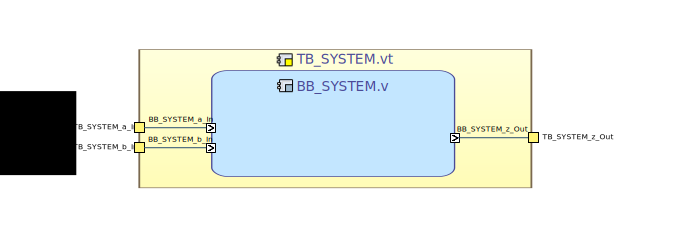
\includegraphics[width=1\linewidth]{\imagesfolderGateAND/GateAND/BB_GateAND.jpg}%
		\end{center}
%#######################################################################
%#######################################################################
%% Funcionalidad: ecuación característica y/o tabla de verdad y/o macro algoritmo general
%#######################################################################
%#######################################################################
\subsection{Funcionalidad}\index{Funcionalidad}
\scriptsize
	\begin{tcolorbox}[enhanced,title=PRODUCTO DE CALIDAD:,colframe=colorA1,colback=colorA2,arc=0mm,colbacktitle=white,fonttitle=\bfseries,coltitle=white,attach boxed title to top left={xshift=3.2mm,yshift=-0.50mm},boxed title style={skin=enhancedfirst jigsaw,size=small,arc=0mm,bottom=1mm,interior style={fill=none,top color=color2,bottom color=color2},,boxrule=0pt},boxrule=0pt]
		OBJETIVO PEDAGÓGICO: El estudiante es capaz de proponer macroalgoritmos descomponiendo el problema en un conjunto de pasos para detallar la funcionalidad esperada del componente. \\
		ENTREGABLES: Ecuación / Tabla de Verdad / Macro-algoritmo correcto y completo según funcionalidad del componente.
		\begin{enumerate}
			\item[a.] El macro-algoritmo de solución describe correctamente la funcionalidad del producto y se representa adecuadamente con una explicación detallada en donde cada paso es menos complejo que el producto solicitado. 
			\item[b.] En cada paso del macro-algoritmo se detalla correctamente un pseudo-algoritmo que describe una posible implementación.
		\end{enumerate}
	\end{tcolorbox}

\normalsize
	%-----------------------------------------------------------------------
		\begin{remark}
			\textbf{Ecuación característica}
		\end{remark}
		\begin{center}	
			\textit{CC\_GateAND\_z\_Out} \textcolor{red}{<=} \textit{CC\_GateAND\_a\_In} \textcolor{red}{and} \textit{CC\_GateAND\_a\_In}; \\
		\end{center}
	%-----------------------------------------------------------------------
		\begin{remark}
			\textbf{Tabla de verdad}
		\end{remark}
		\begin{center}	
			\begin{tabular}{|c|c|c|}
			\hline
			\multicolumn{2}{|c|}{\cellcolor{colorIN1}\textbf{INPUTS}} & \multicolumn{1}{c|}{\cellcolor{colorOUT1}\textbf{OUTPUTS}} \\ \hline
			\cellcolor{colorIN1}\textbf{CC\_GateAND\_a\_In} 	& \cellcolor{colorIN1}\textbf{CC\_GateAND\_b\_In} 	& 	\cellcolor{colorOUT1} \textbf{CC\_GateAND\_z\_Out}	\\ \hline
			\cellcolor{colorIN2} 0								& \cellcolor{colorIN2} 0							& 	\cellcolor{colorOUT2} 0								\\ \hline
			\cellcolor{colorIN2} 0								& \cellcolor{colorIN2} 1							& 	\cellcolor{colorOUT2} 0								\\ \hline
			\cellcolor{colorIN2} 1								& \cellcolor{colorIN2} 0							& 	\cellcolor{colorOUT2} 0								\\ \hline
			\cellcolor{colorIN2} 1								& \cellcolor{colorIN2} 1							& 	\cellcolor{colorOUT2} 1								\\ \hline
			\end{tabular}
		\end{center}
	%-----------------------------------------------------------------------
		\begin{remark}
			\textbf{Macro algoritmo}
		\end{remark}
			\begin{algorithm}[H]
			\SetAlgoLined
				\KwData{$CC\_GateAND\_a\_In$, $CC\_GateAND\_b\_In$ ~(0, 1)}
				\KwResult{$CC\_GateAND\_z\_Out$ ~(0, 1)}
			%initialization\;
					$CC\_GateAND\_z\_Out$ \textcolor{red}{=} $CC\_GateAND\_a\_In$ \textcolor{red}{and} $CC\_GateAND\_b\_In$
				\caption{Compuerta lógica AND}
			\end{algorithm}

		\begin{center}
			\includegraphics[width=0.5\linewidth]{\imagesfolderGateAND/GateAND/FC_GateAND_1.jpg}%
		\end{center}
	%-----------------------------------------------------------------------
%#######################################################################
%#######################################################################
%% HDL: Caja negra
%#######################################################################
%#######################################################################
\subsection{HDL: Caja negra}\index{HDL: Caja negra}
\scriptsize
	\begin{tcolorbox}[enhanced,title=PRODUCTO DE CALIDAD:,colframe=colorA1,colback=colorA2,arc=0mm,colbacktitle=white,fonttitle=\bfseries,coltitle=white,attach boxed title to top left={xshift=3.2mm,yshift=-0.50mm},boxed title style={skin=enhancedfirst jigsaw,size=small,arc=0mm,bottom=1mm,interior style={fill=none,top color=color2,bottom color=color2},,boxrule=0pt},boxrule=0pt]
		OBJETIVO PEDAGÓGICO: El estudiante es capaz de describir lo solicitado en lenguajes de HDL para identificar los elementos básicos de la herramienta de diseño y del lenguaje. \\
		ENTREGABLES: Códigos fuente.
		\begin{enumerate}
			\item[a.] La descripción en lenguajes hardware (complejidad del código, diferencia combinacional y secuencial) es correcta y corresponde al producto solicitado.
			\item[b.] Se incluye documentación completa para estructurar y/o entender el código claramente (indentación y sintaxis de los lenguajes), nombrando correcta y adecuadamente todas las señales, variables y demás elementos relevantes. 
		\end{enumerate}
	\end{tcolorbox}

\normalsize

	%-----------------------------------------------------------------------
	\lstinputlisting[language=Verilog,caption=BB\_SYSTEM.v]{\verilogfolderGateAND/PRJ0_GateAND_1/BB_SYSTEM.v1BB}
	%-----------------------------------------------------------------------
%#######################################################################
%#######################################################################
%% Definición vectores de prueba
%#######################################################################
%#######################################################################
\subsection{Definición vectores de prueba}\index{Definición vectores de prueba}
\scriptsize
	\begin{tcolorbox}[enhanced,title=PRODUCTO DE CALIDAD:,colframe=colorA1,colback=colorA2,arc=0mm,colbacktitle=white,fonttitle=\bfseries,coltitle=white,attach boxed title to top left={xshift=3.2mm,yshift=-0.50mm},boxed title style={skin=enhancedfirst jigsaw,size=small,arc=0mm,bottom=1mm,interior style={fill=none,top color=color2,bottom color=color2},,boxrule=0pt},boxrule=0pt]
		OBJETIVO PEDAGÓGICO: El estudiante es capaz de proponer una estrategia de identificación de vectores de prueba para validar la funcionalidad del componente.\\
		ENTREGABLES: Estrategias claras de selección. Explicación clara de funcionamiento.
		\begin{enumerate}
			\item[a.] Los vectores de prueba se seleccionan a partir de una estrategia explícita y claramente definida expresada en un párrafo. Estos vectores permiten comprobar totalmente la funcionalidad del componente. Se realizan simulaciones funcionales que validan esos vectores de prueba. 
		\end{enumerate}
	\end{tcolorbox}

\normalsize

	En este caso como son pocas entradas se debe validar toda la tabla de verdad. Los vectores de prueba corresponden entonces a dichas combinaciones así:
		\begin{center}
			\begin{tabular}{|c|c|c|}
			\hline
			\multicolumn{2}{|c|}{\cellcolor{colorIN1}\textbf{INPUTS}} & \multicolumn{1}{c|}{\cellcolor{colorOUT1}\textbf{OUTPUTS}} \\ \hline
			\cellcolor{colorIN1}\textbf{CC\_GateAND\_a\_In} 	& \cellcolor{colorIN1}\textbf{CC\_GateAND\_b\_In} 	& 	\cellcolor{colorOUT1} \textbf{CC\_GateAND\_z\_Out}	\\ \hline
			\cellcolor{colorIN2} 0								& \cellcolor{colorIN2} 0							& 	\cellcolor{colorOUT2} ?								\\ \hline
			\cellcolor{colorIN2} 0								& \cellcolor{colorIN2} 1							& 	\cellcolor{colorOUT2} ?								\\ \hline
			\cellcolor{colorIN2} 1								& \cellcolor{colorIN2} 0							& 	\cellcolor{colorOUT2} ?								\\ \hline
			\cellcolor{colorIN2} 1								& \cellcolor{colorIN2} 1							& 	\cellcolor{colorOUT2} ?								\\ \hline
			\end{tabular}
		\end{center}

%#######################################################################
%#######################################################################
%% HDL: Vectores de prueba
%#######################################################################
%#######################################################################
\subsection{HDL: Vectores de prueba}\index{HDL: Vectores de prueba}
\scriptsize
	\begin{tcolorbox}[enhanced,title=PRODUCTO DE CALIDAD:,colframe=colorA1,colback=colorA2,arc=0mm,colbacktitle=white,fonttitle=\bfseries,coltitle=white,attach boxed title to top left={xshift=3.2mm,yshift=-0.50mm},boxed title style={skin=enhancedfirst jigsaw,size=small,arc=0mm,bottom=1mm,interior style={fill=none,top color=color2,bottom color=color2},,boxrule=0pt},boxrule=0pt]
		OBJETIVO PEDAGÓGICO: El estudiante es capaz de describir lo solicitado en lenguajes de HDL para identificar los elementos básicos de la herramienta de diseño y del lenguaje. \\
		ENTREGABLES: Códigos fuente.
		\begin{enumerate}
			\item[a.] La descripción en lenguajes hardware (complejidad del código, diferencia combinacional y secuencial) es correcta y corresponde al producto solicitado.
			\item[b.] Se incluye documentación completa para estructurar y/o entender el código claramente (indentación y sintaxis de los lenguajes), nombrando correcta y adecuadamente todas las señales, variables y demás elementos relevantes. 
		\end{enumerate}
	\end{tcolorbox}

\normalsize

	%-----------------------------------------------------------------------
	\lstinputlisting[language=Verilog,caption=TB\_SYSTEM.vt]{\verilogfolderGateAND/PRJ0_GateAND_1/simulation/modelsim/TB_SYSTEM.vt1}
	%-----------------------------------------------------------------------
%#######################################################################
%#######################################################################
%% Diagrama caja blanca
%#######################################################################
%#######################################################################
\subsection{Diagrama caja blanca}\index{Diagrama caja blanca}
\scriptsize
	\begin{tcolorbox}[enhanced,title=PRODUCTO DE CALIDAD:,colframe=colorA1,colback=colorA2,arc=0mm,colbacktitle=white,fonttitle=\bfseries,coltitle=white,attach boxed title to top left={xshift=3.2mm,yshift=-0.50mm},boxed title style={skin=enhancedfirst jigsaw,size=small,arc=0mm,bottom=1mm,interior style={fill=none,top color=color2,bottom color=color2},,boxrule=0pt},boxrule=0pt]
		OBJETIVO PEDAGÓGICO: El estudiante es capaz de realizar un diagrama con sub-componentes, señales e interconexiones para mostrar un diseño estructurado que permita llegar a una implementación del componente.\\
		ENTREGABLES: Diagrama de sub-componentes, señales e interconexiones, descripción de componente o componente a componente.
		\begin{enumerate}
			\item[a.] El diagrama de caja blanca es correcto y corresponde con el componente solicitado. 
			\item[b.] Se muestran todas las señales de entrada/salida e internas con sus correspondientes nombres estructurados (In/Out) y tamaños (Bit/Bus) para todos los componentes internos del sistema.
			\item[c.] El diagrama de caja blanca corresponde a una solución eficiente en cuanto a recursos, número de bloques y elementos y algoritmo de solución. Los componentes internos son menos complejos que los de mayor jerarquía.
			\item[d.] Se presenta una descripción (qué es y cómo funciona) de cada uno de los componentes constitutivos del componente solicitado, describiendo sus señales.
		\end{enumerate}
	\end{tcolorbox}

\normalsize

		En este caso el diagrama corresponde solamente a la compuerta.
		\begin{center}
			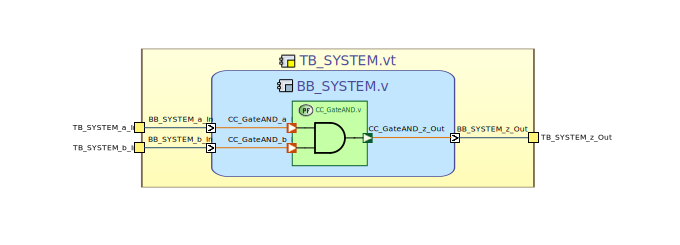
\includegraphics[width=1\linewidth]{\imagesfolderGateAND/GateAND/WB_GateAND.jpg}
		\end{center}
%#######################################################################
%#######################################################################
%% HDL: Caja blanca
%#######################################################################
%#######################################################################
\subsection{HDL: Caja blanca}\index{HDL: Caja blanca}
\scriptsize
	\begin{tcolorbox}[enhanced,title=PRODUCTO DE CALIDAD:,colframe=colorA1,colback=colorA2,arc=0mm,colbacktitle=white,fonttitle=\bfseries,coltitle=white,attach boxed title to top left={xshift=3.2mm,yshift=-0.50mm},boxed title style={skin=enhancedfirst jigsaw,size=small,arc=0mm,bottom=1mm,interior style={fill=none,top color=color2,bottom color=color2},,boxrule=0pt},boxrule=0pt]
		OBJETIVO PEDAGÓGICO: El estudiante es capaz de describir lo solicitado en lenguajes de HDL para identificar los elementos básicos de la herramienta de diseño y del lenguaje. \\
		ENTREGABLES: Códigos fuente.
		\begin{enumerate}
			\item[a.] La descripción en lenguajes hardware (complejidad del código, diferencia combinacional y secuencial) es correcta y corresponde al producto solicitado.
			\item[b.] Se incluye documentación completa para estructurar y/o entender el código claramente (indentación y sintaxis de los lenguajes), nombrando correcta y adecuadamente todas las señales, variables y demás elementos relevantes.  
		\end{enumerate}
	\end{tcolorbox}

\normalsize

	%-----------------------------------------------------------------------
	\lstinputlisting[language=Verilog,caption=BB\_SYSTEM.v]{\verilogfolderGateAND/PRJ0_GateAND_1/BB_SYSTEM.v1WB}
	%-----------------------------------------------------------------------
%#######################################################################
%#######################################################################
%% HDL: bloques
%#######################################################################
%#######################################################################
\subsection{HDL: bloques}\index{HDL: bloques}
\scriptsize
	\begin{tcolorbox}[enhanced,title=PRODUCTO DE CALIDAD:,colframe=colorA1,colback=colorA2,arc=0mm,colbacktitle=white,fonttitle=\bfseries,coltitle=white,attach boxed title to top left={xshift=3.2mm,yshift=-0.50mm},boxed title style={skin=enhancedfirst jigsaw,size=small,arc=0mm,bottom=1mm,interior style={fill=none,top color=color2,bottom color=color2},,boxrule=0pt},boxrule=0pt]
		OBJETIVO PEDAGÓGICO: El estudiante es capaz de describir lo solicitado en lenguajes de HDL para identificar los elementos básicos de la herramienta de diseño y del lenguaje. \\
		ENTREGABLES: Códigos fuente.
		\begin{enumerate}
			\item[a.] La descripción en lenguajes hardware (complejidad del código, diferencia combinacional y secuencial) es correcta y corresponde al producto solicitado.
			\item[b.] Se incluye documentación completa para estructurar y/o entender el código claramente (indentación y sintaxis de los lenguajes), nombrando correcta y adecuadamente todas las señales, variables y demás elementos relevantes. 
		\end{enumerate}
	\end{tcolorbox}

\normalsize

	%-----------------------------------------------------------------------
	\lstinputlisting[language=Verilog,caption=CC\_GateAND.v]{\verilogfolderGateAND/PRJ0_GateAND_1/rtl/CC_GateAND.v1}
	%-----------------------------------------------------------------------
%#######################################################################
%#######################################################################
%% Simulación temporal
%#######################################################################
%#######################################################################
\subsection{Simulación temporal}\index{Simulación temporal}
\scriptsize
	\begin{tcolorbox}[enhanced,title=PRODUCTO DE CALIDAD:,colframe=colorA1,colback=colorA2,arc=0mm,colbacktitle=white,fonttitle=\bfseries,coltitle=white,attach boxed title to top left={xshift=3.2mm,yshift=-0.50mm},boxed title style={skin=enhancedfirst jigsaw,size=small,arc=0mm,bottom=1mm,interior style={fill=none,top color=color2,bottom color=color2},,boxrule=0pt},boxrule=0pt]
	OBJETIVO PEDAGÓGICO: El estudiante es capaz de relacionar la funcionalidad según las especificaciones propuestas con diversos tipos de pruebas para comprobar el funcionamiento del componente según lo solicitado. \\
	ENTREGABLES: Diagramas temporales donde se demuestre funcionalidad según las especificaciones propuestas y en diversos tipos de pruebas.
		\begin{enumerate}
			\item[a.] Se presentan resultados de simulación para el producto solicitado, explicando tres o más casos de funcionamiento sobre el diagrama de simulación. La simulación contiene marcadores en la gráfica que señalan situaciones específicas del producto.
		\end{enumerate}
	\end{tcolorbox}

\normalsize

A continuación se presenta un diagrama de lo que se espera obtener del sistema. En este caso que es sencillo se puede hacer un diagrama de tiempos inicial para ver el comportamiento esperado.

		\begin{tikztimingtable}
			\\ % Gives vertical space
			$CC\_GateAND\_a\_In$	& 2L 2H 2L 2H 2L 2H 2L 2H 2L \\ % starts with edge
			$CC\_GateAND\_b\_In$	& 2L 2L 2H 2H 2L 2L 2H 2H 2L \\ % starts with edge
			\\ % Gives vertical space
			$CC\_GateAND\_z\_Out$	&	2L 2L 2L 2H 2L 2L 2L 2H 2L\\
			\extracode
			%~ \begin{scope}[on background layer]
				%~ \vertlines[help lines,opacity=0.3]{}
			%~ \end{scope}
			\begin{pgfonlayer}{background}
				\vertlines[help lines, dotted]{0,2,...,18}
				\foreach \i [count=\col from 0] in {0,2,...,18}
				\node[font=\scriptsize] at (\i,2) {$t_{\col}$};
				\end{pgfonlayer}
		\end{tikztimingtable}

Por otro lado, se presenta el diagrama de tiempos obtenido en la herramienta Quartus de Altera. En este caso podemos ver como coincide con lo esperado. Es muy importante resaltar los casos de simulación, marcando los vectores de prueba en los resultados de simulación.

		\begin{center}
			\includegraphics[width=1\linewidth]{\imagesfolderGateAND/GateAND/ST_GateAND.pdf}%
		\end{center}
%#######################################################################
%#######################################################################
%% Diagramas QUARTUS
%#######################################################################
%#######################################################################
\subsection{Diagramas QUARTUS}\index{Diagramas QUARTUS}
\scriptsize
	\begin{tcolorbox}[enhanced,title=PRODUCTO DE CALIDAD:,colframe=colorA1,colback=colorA2,arc=0mm,colbacktitle=white,fonttitle=\bfseries,coltitle=white,attach boxed title to top left={xshift=3.2mm,yshift=-0.50mm},boxed title style={skin=enhancedfirst jigsaw,size=small,arc=0mm,bottom=1mm,interior style={fill=none,top color=color2,bottom color=color2},,boxrule=0pt},boxrule=0pt]
		OBJETIVO PEDAGÓGICO: El estudiante es capaz de identificar elementos de la Herramienta Quartus para comprender mejor el proceso de diseño.\\
		ENTREGABLES: Diagramas obtenidos en la herramienta.
		\begin{enumerate}
			\item[a.] Se presentan diagramas obtenidos por QUARTUS.
		\end{enumerate}
	\end{tcolorbox}

\normalsize

		\begin{center}
			\includegraphics[width=1\linewidth]{\imagesfolderGateAND/GateAND/Q_GateAND.pdf}%
		\end{center}
%#######################################################################
%#######################################################################
%% Resultados y lecciones aprendidas
%#######################################################################
%#######################################################################
\subsection{Resultados y lecciones aprendidas}\index{Resultados y lecciones aprendidas}
\scriptsize
	\begin{tcolorbox}[enhanced,title=PRODUCTO DE CALIDAD:,colframe=colorA1,colback=colorA2,arc=0mm,colbacktitle=white,fonttitle=\bfseries,coltitle=white,attach boxed title to top left={xshift=3.2mm,yshift=-0.50mm},boxed title style={skin=enhancedfirst jigsaw,size=small,arc=0mm,bottom=1mm,interior style={fill=none,top color=color2,bottom color=color2},,boxrule=0pt},boxrule=0pt]
		OBJETIVO PEDAGÓGICO: El estudiante es capaz de discutir el proceso de diseño para evidenciar problemas, mejoras del componente diseñado.\\
		ENTREGABLES: Contiene máximo dos párrafos (claros, precisos y coherentes).
		\begin{enumerate}
			\item[a.] Se proponen nuevas especificaciones y aplicaciones del trabajo realizado (ejemplo: mayores niveles de complejidad y usos en otros contextos).
			\item[b.] En caso de no lograr el item de funcionamiento glogal; identifica y argumenta las razones principales del no funcionamiento. 
			\item[c.] El lenguaje disciplinar es preciso y adecuado, haciendo uso de frases gramaticalmente correctas, sin errores ortográficos.
		\end{enumerate}
	\end{tcolorbox}

\normalsize

	\begin{tcolorbox}[colback=colorT2,colframe=colorT1,arc=0mm,boxrule=0pt,title=]
		La compuerta lógica AND es uno de los elementos más simples de la electrónica digital y se pude implementar a partir de su ecuación lógica. Además, se pueden realizar una descripción a nivel funcional como se va presentar en la siguiente sección. \\
	\end{tcolorbox}

	\newpage
	


%#######################################################################
%#######################################################################
%% Componente
%#######################################################################
%#######################################################################
\section{Componente}\index{Componente}
\normalsize
A continuación se presenta el componente \textbf{componente} mostrando su descripción ...
%#######################################################################
%#######################################################################
%% Descripción del componente
%#######################################################################
%#######################################################################
\subsection{Descripción del componente}\index{Descripción del componente}
%#######################################################################
\scriptsize

%#######################################################################
\normalsize

	El componente ...
%#######################################################################
%#######################################################################
%% Símbolo
%#######################################################################
%#######################################################################
\subsection{Símbolo}\index{Símbolo}
%#######################################################################
\scriptsize

%#######################################################################
\normalsize

	El componente ...
%#######################################################################
%#######################################################################
%% Diagrama caja negra
%#######################################################################
%#######################################################################
\subsection{Diagrama caja negra}\index{Diagrama caja negra}
%#######################################################################
\scriptsize

%#######################################################################
\normalsize

	El componente ...
%#######################################################################
%#######################################################################
%% Funcionalidad: ecuación característica y/o tabla de verdad y/o macro algoritmo general
%#######################################################################
%#######################################################################
\subsection{Funcionalidad}\index{Funcionalidad}
%#######################################################################
\scriptsize

%#######################################################################
\normalsize

	El componente ...
%#######################################################################
%#######################################################################
%% HDL: Caja negra
%#######################################################################
%#######################################################################
\subsection{HDL: Caja negra}\index{HDL: Caja negra}
%#######################################################################
\scriptsize

%#######################################################################
\normalsize

	El componente ...
%#######################################################################
%#######################################################################
%% Definición vectores de prueba
%#######################################################################
%#######################################################################
\subsection{Definición vectores de prueba}\index{Definición vectores de prueba}
%#######################################################################
\scriptsize

%#######################################################################
\normalsize

	El componente ...
%#######################################################################
%#######################################################################
%% HDL: Vectores de prueba
%#######################################################################
%#######################################################################
\subsection{HDL: Vectores de prueba}\index{HDL: Vectores de prueba}
%#######################################################################
\scriptsize

%#######################################################################
\normalsize

	El componente ...
%#######################################################################
%#######################################################################
%% Diagrama caja blanca
%#######################################################################
%#######################################################################
\subsection{Diagrama caja blanca}\index{Diagrama caja blanca}
%#######################################################################
\scriptsize

%#######################################################################
\normalsize

	El componente ...
%#######################################################################
%#######################################################################
%% HDL: Caja blanca
%#######################################################################
%#######################################################################
\subsection{HDL: Caja blanca}\index{HDL: Caja blanca}
%#######################################################################
\scriptsize

%#######################################################################
\normalsize

	El componente ...
%#######################################################################
%#######################################################################
%% HDL: bloques
%#######################################################################
%#######################################################################
\subsection{HDL: bloques}\index{HDL: bloques}
%#######################################################################
\scriptsize

%#######################################################################
\normalsize

	El componente ...
%#######################################################################
%#######################################################################
%% Simulación temporal
%#######################################################################
%#######################################################################
\subsection{Simulación temporal}\index{Simulación temporal}
%#######################################################################
\scriptsize

%#######################################################################
\normalsize

	El componente ...
%#######################################################################
%#######################################################################
%% Diagramas QUARTUS
%#######################################################################
%#######################################################################
\subsection{Diagramas QUARTUS}\index{Diagramas QUARTUS}
%#######################################################################
\scriptsize

%#######################################################################
\normalsize

	El componente ...
%#######################################################################
%#######################################################################
%% Resultados y lecciones aprendidas
%#######################################################################
%#######################################################################
\subsection{Resultados y lecciones aprendidas}\index{Resultados y lecciones aprendidas}
%#######################################################################
\scriptsize

%#######################################################################
\normalsize

	El componente ...



%----------------------------------------------------------------------------------------
%	BIBLIOGRAPHY
%----------------------------------------------------------------------------------------
%~ \chapter*{Bibliography}
%~ \addcontentsline{toc}{chapter}{\textcolor{ocre}{Bibliography}}
%~ \section*{Books}
%~ \addcontentsline{toc}{section}{Books}
%~ \printbibliography[heading=bibempty,type=book]
%~ \section*{Articles}
%~ \addcontentsline{toc}{section}{Articles}
%~ \printbibliography[heading=bibempty,type=article]
%----------------------------------------------------------------------------------------
%	INDEX
%----------------------------------------------------------------------------------------
%~ \cleardoublepage
%~ \phantomsection
%~ \setlength{\columnsep}{0.75cm}
%~ \addcontentsline{toc}{chapter}{\textcolor{ocre}{Index}}
%~ \printindex

%----------------------------------------------------------------------------------------

\end{document}
